\documentclass[12pt,a4paper]{article}

\usepackage[T1]{fontenc}
\usepackage[utf8]{inputenc}
\usepackage{graphicx}
\usepackage{float}
\usepackage{geometry}
\usepackage{listings}
\usepackage{xcolor}
\usepackage{fancyhdr}
\usepackage{amsmath}
\usepackage{amssymb}
\usepackage{booktabs}
\usepackage{caption}
\usepackage{needspace}
\usepackage{array}
\usepackage{tikz}
\usetikzlibrary{arrows.meta,positioning,shapes.geometric}

\AddToHook{cmd/subsection/before}{\Needspace{5\baselineskip}}

\geometry{margin=1in}
\captionsetup{font=small,labelfont=bf}
\setlength{\textfloatsep}{14pt}
\setlength{\emergencystretch}{2em}

\lstdefinestyle{mystyle}{
    language=Python,
    basicstyle=\ttfamily\footnotesize,
    breaklines=true,
    columns=fullflexible,
    keepspaces=true,
    showstringspaces=false,
    xleftmargin=1.5em,
    numbers=left,
    numberstyle=\tiny,
    keywordstyle=\color{blue},
    commentstyle=\color{green!50!black},
    stringstyle=\color{red}
}
\lstset{style=mystyle}

% Pseudocode: plain listings with math, so no extra package is needed
\newcommand{\kw}[1]{\textbf{#1}}
\lstdefinestyle{pseudostyle}{
    language={},
    basicstyle=\normalfont\small,
    mathescape=true,
    escapeinside={(*}{*)},
    columns=fullflexible,
    keepspaces=true,
    breaklines=true,
    numbers=left,
    numberstyle=\tiny,
    xleftmargin=1.5em,
    frame=tb,
    tabsize=3
}
\DeclareCaptionType[fileext=loa]{algo}[Algorithm]

\setlength{\headheight}{15pt}
\pagestyle{fancy}
\fancyhf{}
\fancyhead[L]{Energy-Optimal Control of the UR5e}
\fancyhead[R]{Project Report}
\fancyfoot[C]{\thepage}

% Flowchart styles
\tikzset{
    fbox/.style={draw=magenta!80!black, fill=magenta!6, thick, minimum width=5.6cm,
                 minimum height=0.8cm, align=center, font=\small},
    fnew/.style={fbox, draw=green!50!black, fill=green!12},
    fdec/.style={draw=magenta!80!black, fill=white, thick, diamond, aspect=2,
                 inner sep=1pt, align=center, font=\small},
    fstart/.style={draw=magenta!80!black, fill=magenta!6, thick, ellipse,
                   minimum width=3cm, minimum height=0.8cm, font=\small},
    flow/.style={-{Stealth[length=2.2mm]}, thick, draw=magenta!80!black},
    flabel/.style={font=\footnotesize, text=magenta!80!black}
}

\begin{document}

% =========================================================
% TITLE PAGE
% =========================================================
\begin{titlepage}
\centering

\vspace*{4cm}
{\LARGE \textbf{Energy-Optimal Control of the UR5e\\[0.2cm] for Soda-Can Packing}}\\[0.6cm]
{\large Project Report}\\

\vspace{3cm}
{\Large \textbf{Authors}}\\[0.3cm]
{\large Ahmed Hamouda}\\[0.1cm]
{\large Zainab Almagbari}\\

\vfill
{\large November 2026}
\end{titlepage}

\section{Project flowchart}

A UR5e packs soda cans from a conveyor into a $3\times4$ carton in a Gazebo and ROS~2 simulation, at a fixed rhythm of one can every 22~s. Figure~\ref{fig:flow} is the project flowchart. The green boxes are the steps this project adds: the existing controllers tested are the ones in the UR5e ROS~2 stack, an energy metric step was added, and the comparison uses energy instead of tracking error.

\begin{figure}[H]
\centering
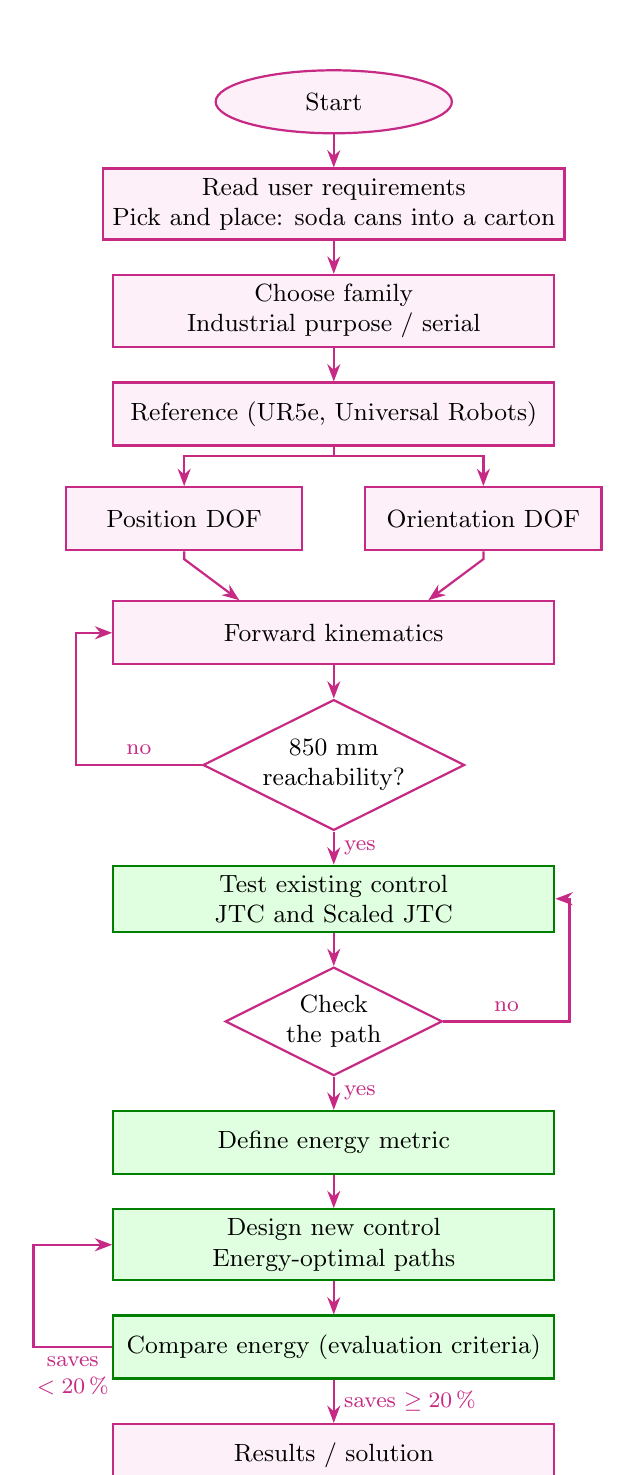
\begin{tikzpicture}[node distance=0.42cm]
\node[fstart] (start) {Start};
\node[fbox, below=of start] (req) {Read user requirements\\Pick and place: soda cans into a carton};
\node[fbox, below=of req] (fam) {Choose family\\Industrial purpose / serial};
\node[fbox, below=of fam] (ref) {Reference (UR5e, Universal Robots)};
\node[fbox, minimum width=3cm, below=0.5cm of ref, xshift=-1.9cm] (pos) {Position DOF};
\node[fbox, minimum width=3cm, below=0.5cm of ref, xshift=1.9cm] (ori) {Orientation DOF};
\node[fbox, below=1.95cm of ref] (fk) {Forward kinematics};
\node[fdec, below=of fk] (reach) {850 mm\\reachability?};
\node[fnew, below=of reach] (test) {Test existing control\\JTC and Scaled JTC};
\node[fdec, below=of test] (path) {Check\\the path};
\node[fnew, below=of path] (metric) {Define energy metric};
\node[fnew, below=of metric] (design) {Design new control\\Energy-optimal paths};
\node[fnew, below=of design] (cmp) {Compare energy (evaluation criteria)};
\node[fbox, below=0.55cm of cmp] (res) {Results / solution};

\draw[flow] (start) -- (req);
\draw[flow] (req) -- (fam);
\draw[flow] (fam) -- (ref);
\draw[flow] (ref.south) -- ++(0,-0.12) -| (pos.north);
\draw[flow] (ref.south) -- ++(0,-0.12) -| (ori.north);
\draw[flow] (pos.south) -- ++(0,-0.1) -- ([xshift=-1.2cm]fk.north);
\draw[flow] (ori.south) -- ++(0,-0.1) -- ([xshift=1.2cm]fk.north);
\draw[flow] (fk) -- (reach);
\draw[flow] (reach) -- node[flabel, right] {yes} (test);
\draw[flow] (reach.west) -- node[flabel, above] {no} ++(-1.6,0) |- (fk.west);
\draw[flow] (test) -- (path);
\draw[flow] (path.east) -- node[flabel, above] {no} ++(1.6,0) |- (test.east);
\draw[flow] (path) -- node[flabel, right] {yes} (metric);
\draw[flow] (metric) -- (design);
\draw[flow] (design) -- (cmp);
\draw[flow] (cmp.west) -- node[flabel, below, align=center] {saves\\$<20\,\%$} ++(-1.0,0) |- (design.west);
\draw[flow] (cmp) -- node[flabel, right] {saves $\geq 20\,\%$} (res);
\end{tikzpicture}
\caption{Project flowchart. Green: the steps this project adds.}
\label{fig:flow}
\end{figure}

\section{Important parts of the code}

The code is the \texttt{ur5e\_pp\_control} ROS~2 package. The listings below are copied from it.

\subsection{Energy model}

The energy of a motion comes from the UR5e motor model of Clochiatti et al.\ (\textit{Robotica}, 2024). The first term is the mechanical power and the second is the motor heat, which is also paid when the arm holds still:
\begin{equation}
P_i = \frac{k_b}{k_t}\,\tau_i\dot q_i + \frac{\tau_i^2}{(N k_{m,i})^2},
\qquad
E = \int \max\Big(0, \sum_i P_i\Big)\,dt .
\end{equation}
The torque $\tau = M(q)\ddot q + C(q,\dot q)\dot q + g(q)$ comes from the inverse dynamics model in \texttt{dynamics.py}, because the torque Gazebo reports contains only the gravity part.

\begin{lstlisting}[caption={Motor constants and power (\texttt{validate.py})}]
GEAR = 100.0
KM = np.array([0.27426] * 3 + [0.06632] * 3)       # Nm/sqrt(W)
KB_OVER_KT = 1.0 / 0.89
C_CU = 1.0 / (GEAR * KM) ** 2                      # W per (N.m)^2 of joint torque

def power(tau, qd):
    """Per-joint electrical, mechanical and copper power, shape (N, 6)."""
    mech = tau * qd
    cu = C_CU * tau ** 2
    return KB_OVER_KT * mech + cu, mech, cu
\end{lstlisting}

\subsection{Path builder}

Inverse kinematics runs only at 9 key poses. Between them, each joint follows a spline with minimum-jerk timing, so $q$, $\dot q$ and $\ddot q$ are analytic and the velocity and acceleration are zero at every stop.

\begin{lstlisting}[caption={One move of the path (\texttt{energy\_opt.py}, \texttt{Planner.build})}]
if len(knots) == 1:                              # dwell
    q, qd, qdd = np.repeat(knots[0][None], n, 0), np.zeros((n, 6)), np.zeros((n, 6))
else:
    # path q(s), s in [0, 1], through the knots; timing s(t) minimum jerk
    spline = CubicSpline(np.linspace(0, 1, len(knots)), np.array(knots), bc_type='natural')
    s = 10 * tau ** 3 - 15 * tau ** 4 + 6 * tau ** 5
    sd = (30 * tau ** 2 - 60 * tau ** 3 + 30 * tau ** 4) / T
    sdd = (60 * tau - 180 * tau ** 2 + 120 * tau ** 3) / T ** 2
    q, dq, ddq = spline(s), spline(s, 1), spline(s, 2)
    qd = dq * sd[:, None]
    qdd = ddq * sd[:, None] ** 2 + dq * sdd[:, None]
\end{lstlisting}

\subsection{Cost of one candidate motion}

Each candidate is rated by its predicted energy and a penalty for every broken rule. The listing shows the energy and the first two rules. The other rules follow the same pattern.

\begin{lstlisting}[caption={Energy and first rules (\texttt{energy\_opt.py}, \texttt{Planner.evaluate})}]
def evaluate(self, k, dt=0.05):
    """(E_elec, penalty, details) for knob dict k. Penalty 0 means every rule holds."""
    self.n_eval += 1
    tk = self.task
    path = self.build(k, dt)
    if path is None:
        return np.inf, np.inf, {}
    t, q, qd, qdd, seg = path['t'], path['q'], path['qd'], path['qdd'], path['segment']
    carried = np.isin(seg, ATTACHED)
    tau = self.dyn.tau(q, qd, qdd, np.where(carried, tk.box_mass, 0.0))
    P = np.maximum(power(tau, qd)[0].sum(1), 0.0)
    E = float(np.sum(0.5 * (P[1:] + P[:-1]) * np.diff(t)))

tool = np.array([fk_all(qi)[-1][:3, 3] for qi in q])
pen = [max(-path['t_wait'], 0.0) * 10]                                  # motion fits in the takt
v = np.linalg.norm(np.diff(tool, axis=0), axis=1) / np.diff(t)
pen.append(max(v.max() - V_TCP_MAX, 0.0) * 10)                          # TCP speed
\end{lstlisting}

\subsection{Search}

\begin{lstlisting}[caption={Rate all starts, then refine the best (\texttt{energy\_opt.py}, \texttt{Planner.optimize})}]
starts = starts or default_starts(self.task) + coarse_grid(self.task)
best = {'E': np.inf}

def f(x):
    xc = np.clip(x, LO, HI)
    k = dict(zip(KNOBS, xc))
    E, pen, _ = self.evaluate(k, dt)
    if pen == 0 and E < best['E']:
        best.update(E=E, k=k)
        if callback:
            callback(k, E)
    return E + 1000 * pen + 1000 * float(np.sum(np.abs(x - xc)))

x0s = [np.array([k0[n] for n in KNOBS]) for k0 in starts]
rated = sorted(zip([f(x) for x in x0s], range(len(x0s))))       # best first
for _, i in rated[:n_refine]:
    minimize(f, x0s[i], method='Nelder-Mead',
             options=dict(maxfev=max_eval, xatol=1e-4, fatol=1e-3, adaptive=True))
return best.get('k'), best['E']
\end{lstlisting}

\subsection{Using the result on the robot}

The new controller replaces only the reference layer. At the start of each cycle, the runner picks the best path for the current carton slot and sends it to the same trajectory controller.

\begin{lstlisting}[caption={Choosing the path for the next can (\texttt{runner\_node.py})}]
def _start_cycle(self, n):
    self.slot = (n - 1) % len(self.refs)
    if self.scenario == 'cans' and self.slot == 0 and n > 1:
        self._empty_carton()
        self.prev_slot = None
    prev = self.plan_version[self.slot]
    self._take_plan()
    self.ref = self.refs[self.slot]
    if self.plan_version[self.slot] != prev:
        self.get_logger().info(f'cycle {n} (slot {self.slot}): optimized path v{self.plan_version[self.slot]}, '
                               f'predicted {self.plan_E[self.slot]:.2f} J'
                               f'{" (search finished)" if self.search_done else ""}')
\end{lstlisting}

\section{Optimization algorithm}

The search variables are
$\theta = (h,\ \text{transfer via-point},\ \text{return via-point},\ \text{wait pose},\ T_{\text{moves}})$,
where $h$ is the lift height and $T_{\text{moves}}$ are the move durations. The cycle always lasts the takt time $T_{\text{takt}} = 22$~s. If the motion finishes early, the robot waits, and waiting also costs energy. Algorithm~\ref{alg:eval} rates one motion and Algorithm~\ref{alg:opt} finds the best motion for every carton slot.

\noindent\begin{minipage}{\linewidth}
\captionof{algo}{Rate one candidate motion: \textsc{Evaluate}$(\theta)$}\label{alg:eval}
\begin{lstlisting}[style=pseudostyle]
(*\kw{Input:}*) motion $\theta$, task (pick, place, can mass, $T_{\text{takt}}$, obstacles)
(*\kw{Output:}*) energy $E$, penalty $p$
Solve IK at the 9 key poses
(*\kw{if}*) a pose is not reachable (*\kw{then return}*) $E = \infty$, $p = \infty$
$T_{\text{wait}} \leftarrow T_{\text{takt}} - \sum$ (durations of all moves and pauses)
Build $q(t), \dot q(t), \ddot q(t)$: joint splines with minimum-jerk timing, step 50 ms
$\tau(t) \leftarrow M(q)\ddot q + C(q,\dot q)\dot q + g(q)$, adding the can mass while it is carried
$P_i(t) \leftarrow (k_b/k_t)\,\tau_i\dot q_i + \tau_i^2/(N k_{m,i})^2$
$E \leftarrow \int \max(0, \sum_i P_i)\,dt$
Tool path $\leftarrow$ forward kinematics of $q(t)$
$p \leftarrow$ sum of the violations of these rules:
   $T_{\text{wait}} \geq 0$ and tool speed $\leq 0.20$ m/s
   can and gripper at least 1 cm above the table, carton walls, packed cans and next can
   lift and lower vertical, within 3 mm
   tool at least 0.25 m from the base axis
   joint torques within 150 and 28 N$\cdot$m
(*\kw{return}*) $E$, $p$
\end{lstlisting}
\end{minipage}

\vspace{0.8cm}

\noindent\begin{minipage}{\linewidth}
\captionof{algo}{Find the energy-optimal motion of every carton slot}\label{alg:opt}
\begin{lstlisting}[style=pseudostyle]
(*\kw{Input:}*) tasks for slots $1 \dots 12$
(*\kw{Output:}*) best motion $\theta^*_s$ for every slot $s$
(*\kw{for each}*) round (Grid: 0 refinements; Quick: 1 refinement, 200 evaluations; Full: 3 refinements, 1500 evaluations) (*\kw{do}*)
   (*\kw{for each}*) slot $s$ (*\kw{do}*)
      Starts $\leftarrow \theta^*_s$ (if known) + 4 start motions + coarse grid over lift, speed and wait pose
      Cost $f(\theta) = E + 1000\,p$ (+ 1000 $\times$ distance outside the bounds)
      Rate every start with $f$ using (*\textsc{Evaluate}*)
      (*\kw{for each}*) of the best starts, as many as this round's refinements (*\kw{do}*)
         Refine with Nelder-Mead on $f$
      (*\kw{end}*)
      $\theta^*_s \leftarrow$ the valid motion ($p = 0$) with the lowest $E$ seen so far
   (*\kw{end}*)
(*\kw{end}*)
Save all $\theta^*_s$; each cycle, the runner sends the path of its slot to the JTC
\end{lstlisting}
\end{minipage}

\vspace{0.5cm}

\noindent\textbf{Result.} Measured in Gazebo at the same rhythm, the energy per carton of 12 cans fell from 593.3~J to 425.7~J, a saving of 28.3\,\%, above the 20\,\% target. There were no faults, and the maximum tool error was 4.0~mm (3.0~mm before). The mean peak power rose from 11.5~W to 13.7~W.

\end{document}
